\chapter{Calibration and Verification of Quantum Devices}
\label{ch:QCV}
This chapter is a collection of work done for various experiments, all of which
concerns either calibrating a device or verifying the output of the experiment.
I discuss calibration in general terms, and present a case study of calibrating
the bulk optics circuit used for simulations in chapter~\ref{ch:Simulations}
which highlights some important features. My work in calibrating this circuit
formed a large part of the early years of my PhD and was a substantial
contribution to the success of the simulation experiments. After calibrating the
circuit, I performed a randomised benchmarking test to verify correct operation.
I derived the random unitaries for this part of the experiment, and took all
the experimental data. The experimental
circuit was designed and built by Enrique Mart\'in L\'opez and the project was
supervised by Anthony Laing.

A large part of the verification section is based on my contributions to an
experiment published in~\cite{verification}, in which I was one of several
co-authors. In this publication, I performed a Bayesian model analysis on a
\bosonsampling{} experiment and developed the theory of the `bosonic clouding'
phenomenon presented as a general verification procedure. Finally, I present a
similar Bayesian model analysis applied to 6-photon data, which appear in
the preprint~\cite{bigreck}, on which I am one of several co-authors. While I
didn't take any of the data in this section, my analysis forms a substantial
part of both publications mentioned.

\section{Calibration}
\label{sec:Calibration}
Future experiments in linear optics are going to exhibit a high degree of
reconfigurability. Fully programmable integrated optics circuits, based on the
scheme in~\cite{reck} are now being constructed and tested in the
lab~\cite{bigreck, qpp}. An important challenge in using such devices is the
calibration of the components: constructing a map between unitary matrices and
parameters on the circuit. Chapter~\ref{ch:DirectDialling} presents the
mathematical coordinate transformation that applies in the ideal case, but not
in the more realistic scenarios encountered in real devices.

The first step in a calibration is finding the origins for the parameters: we
have
a control \(V\) that affects a reflectivity \(r\) (on integrated optics this is
often a voltage controlling a heater, which controls a phase, which controls the
reflectivity of an MZI) but we do not know a priori what settings of \(V\)
correspond to \(r=0\) and \(r=1\). By scanning over a range of \(V\) and
observing the effect of quantities with a known dependence on \(r\), we can
approximate \(r \of{V}\), as described in \cite{peteschip}. Under these
conditions, the task of calibrating the full circuit is more involved than the
ideal case, but still fairly straightforward since the components are
independent. The automation of this process has been discussed in a slightly
different context (separating orthogonal input states) in~\cite{alignment}.

\begin{figure}[t]
  \centering
  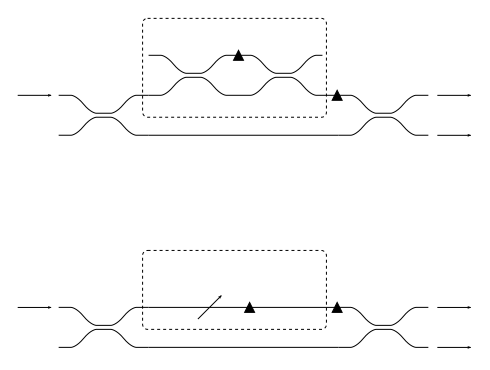
\includegraphics{figures/crosstalk}
  \caption[Nested Mach Zehnder interferometers]
  {Nested Mach Zehnder interferometers. The phase \(\theta\) controlling the
  inner MZI affects both the visibility and the origin of the fringes in the
  outer MZI. We cannot treat the phases and the reflectivities as independent.}
  \label{fig:nestedMZI}
\end{figure}

Up to now, all components in the circuit have been considered independent. I now
continue to discuss the phenomenon of crosstalk, and the implications on the
general calibration problem. A simple example of crosstalk---nested Mach Zehnder
interferometers---is illustrated in figure~\ref{fig:nestedMZI}. In this setup,
we have a generalised Mach Zehnder interferometer (MZI) controlled by a phase
\(\phi\) and a loss \(\eta\) in one arm (b). The loss is implemented with
another MZI, controlled by phase \(\theta\) (a). In an ideal case, the
parameters \(\eta\) and \(\phi\) could be treated independently: scanning over
the range of \(\phi\) would generate interference fringes in the reflectivity of
the outer MZI; the loss \(\eta\) would affect the visibility of the fringe, but
not the origin. In the realistic fringe in figure~\ref{fig:nestedMZI}(c), a
shift of \(\frac{\theta}{2}\) is observed, therefore the assumption of
independence is violated.

A calibration can be achieved by setting the loss \(\eta\) to the desired value,
then setting the phase \(\phi\), taking the shift into account. \(\phi\) must
then be adjusted any time \(\eta\) changes. This situation with nested MZIs is
unavoidable in integrated optics versions of the Reck scheme (see
figure~\ref{fig:ReckScheme}), and can be dealt with in the manner described.
Instead of losses, it is amplitude splittings that crosstalk with the internal
phases, but the effect is the same.

This simple case of crosstalk is not particularly hard to deal with, since its
effect can be precisely predicted in terms of ideal components. I will refer to
this scenario as type I crosstalk. More complicated cases (type II crosstalk)
concern couplings due to imperfect components or
isolation. For example, when using thermal optic phase shifts in integrated
optics, the heaters are not perfectly thermally isolated. Increasing the voltage
on one heater could cause a phase shift in nearby components. In addition to
this, the
voltage controllers for the heaters may not be perfectly electrically isolated:
an increase in one voltage could cause a shift in voltages elsewhere. Unlike the
thermal crosstalk, the effect of electrical crosstalk may not even be
localised. These effects are generally unique to a particular device, and must
be dealt with on a case-by-case basis. I will now discuss a practical example of
calibrating a device in the presence of multiple varieties of crosstalk.

\begin{figure}[t]
  \centering
  \begin{subfigure}{\textwidth}
    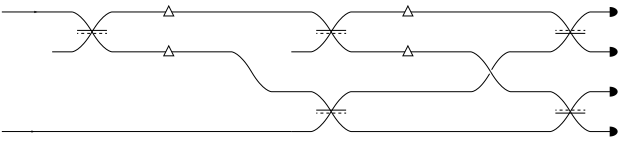
\includegraphics{figures/schematic.pdf}
    \caption{A schematic of the circuit, expanded into path}
    \label{fig:schematic}
  \end{subfigure} \\
  \vspace{1cm}
  \begin{subfigure}{0.45\textwidth}
    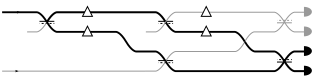
\includegraphics{figures/interferometerAB.pdf}
    \caption{A/B interferometer}
    \label{fig:ab}
  \end{subfigure}
  \hspace{0.05\textwidth}
  \begin{subfigure}{0.45\textwidth}
    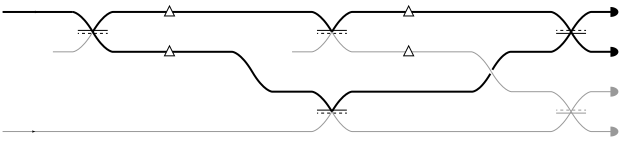
\includegraphics{figures/interferometerCD.pdf}
    \caption{C/D interferometer}
    \label{fig:cd}
  \end{subfigure}
  \caption[Illustration of nested interferometers in the bulk Reck scheme]
  {Path representation of interferometers present in a reconfigurable bulk
  optics circuit. Depending on the settings of the amplitude parameters, two
  different interferometric paths are available.}
  \label{fig:interferometers}
\end{figure}

The device in question is the bulk optics device used for the simulations in
chapter~\ref{ch:Simulations}. For ease of discussion, I have expanded the
path-polarisation description of the circuit in figure~\ref{fig:circuit} into a
path-only equivalent in figure~\ref{fig:schematic}. The waveplates implementing
amplitude splittings (\(at_{0}, at_{1}, aq_{0}, aq_{1}, aq_{2}\)) are shown as
beamsplitters, and the phase shifts implemented by the waveplates \(\phi_{0}\)
and \(\phi_{1}\) are shown on the relevant paths. In figures~\ref{fig:ab}
and~\ref{fig:cd}, I have highlighted the two interferometers, which can produce
fringes in count rates at detectors A and B and detectors C and D respectively.

When \(\phi_{0}\) is scanned, the observed interference fringes are as expected,
but the origin of the fringes shifts as a function of other components in the
interferometer, \(aq_{0}\) and \(at_{1}\), which in the ideal case would have no
effect on the internal phase. This is an example of type I crosstalk, and the
phase shifts due to \(aq_{0}\) and \(at_{1}\) could be characterised through
measurement and incorporated into the calibration. However, due to the nature of
bulk optics, there is generally a further drift in the origin of the fringe due
to movement of components. This drift cannot be characterised, but the timescale
is sufficiently slow that it does not have to be adjusted for in any given run
of the experiment. The approach we used to deal with these effects (drift and
type I crosstalk) was to perform a new phase calibration for every unitary, with
the amplitude splittings \(aq_{0}\) and \(at_{1}\) set, then assume that drift
would be negligible for the time required to take the data. Note that drift is
not an issue in integrated optics \cite{politi-ic}.

Scanning \(\phi_{1}\) results in much more complicated interference fringes,
shown in figure~\ref{fig:crapusoid}, due to type II crosstalk (self crosstalk in
this case). To understand the strange shape of this interference fringe, we
need to consider how the phase is
implemented by a waveplate acting on polarisation degrees of freedom. As shown
in figure~\ref{fig:circuit}, the phase shift is achieved by a series of three
waveplates: a half waveplate at an angle \(2\phi_{1}\) between two quarter
waveplates at \(45\deg\). Two modes (one horizontal and one vertical
polarisation) pass
through all three waveplates, collecting a relative phase of \(2\phi_{1}\) and
two other modes (again, one horizontal and one vertical polarisation) pass only
through the two
quarter waveplates, flipping horizontal to vertical and vice versa. The
crosstalk effect is derived from the fact that the two modes passing through the
half waveplate both collect an additional phase with respect to the two modes
that do not, which depends on the angle of the half waveplate. This is all
represented schematically in figure~\ref{fig:schematic} by the phases \(\delta
\of{\phi_{1}} + \phi_{1}\) and \(\delta \of{\phi_{1}} - \phi_{1}\) on the upper
two modes. The lower two modes do not pass through the half waveplate so collect
no phase.

\begin{figure}[h]
  \centering
  \includegraphics{figures/crapusoid}
  \caption[Interference fringes distorted by crosstalk between components]
  {Interference fringes observed in the bulk optics circuit. The distortion of
  the fringes is not due to an imperfect waveplate implementing the phase shift,
  but a kind of crosstalk between components. In this instance, the circuit
  parameters were set to \(at_{0}=22.5\deg\), \(at_{1}=24.45\deg\),
  \(aq_{0}=20.95\deg\), \(aq_{1}=22.5\deg\), \(aq_{2}=22.5\deg\). The waveplate
  controlling \(\phi_{0}\) was fixed and the waveplate controlling \(\phi_{2}\)
  was scanned for a full rotation. Lines are fitted to the data using
  equation~\ref{eq:crapusoid}.}
  \label{fig:crapusoid}
\end{figure}

The function \(\delta \of{\phi_{1}}\) is sinusoidal, and we can model the
count rates in figure~\ref{fig:crapusoid} using the function
\begin{equation}
  \label{eq:crapusoid}
  C \of{\phi_{1}} = A \left[ 1 \pm \cos \of{ \phi_{1} - \beta - \varepsilon
  \cos \of{ \phi_{1} - r}} \right] + d
\end{equation}
Fitting the data to this function, we can effectively calibrate the device in
the presence of the type II crosstalk. 

\section{Randomised benchmarking}
\label{sec:Benchmarking}
In order to test the calibration of the bulk optics circuit, we used it to
implement a series of Haar random unitaries: a process known as randomised
benchmarking. This testing procedure (also seen, for example,
in~\cite{peteschip}) is popular when the device being tested exhibits a high
degree of reconfigurability. By taking random samples throughout the entire
parameter space, we gain a degree of confidence that the device will work well
in any configuration.

The data taken consist of single photon detection statistics and two photon
correlations. For the single photon data, we can inject in two possible input
modes, and measure in four outputs (A, B, C, D), giving us two probability
distributions, each of four elements. I refer to these as the \emph{quart}
and \emph{trit} distributions, with the elements \(\vec{q}= \left( q_{A}, q_{B},
q_{C}, q_{D} \right)\) and \(\vec{t} = \left( t_{A}, t_{B}, t_{C}, t_{D}
\right)\) respectively. Subscripts refer to the detector label. Coincidences are
counted between all pairs of detectors (AB, AC, AD, BC, BD, CD), but here there
is only one input configuration. However, a delay can be introduced between
the two photons, giving us two possible probability distributions each with six
elements, which I refer to as quantum (\(\vec{Q}\)) for no temporal delay and
classical (\(\vec{C}\)) for a large temporal delay. Since the detectors are not
number resolving, we cannot measure the two photon events with multiple
occupancy, so these distributions are not normalised. A comparison of the
measured distributions to the expected distributions is illustrated in
figure~\ref{fig:benchmarking} for a single random matrix.

\begin{figure}[t]
  \includegraphics{figures/benchmarking}
  \caption[Sample data from randomised benchmarking]
  {Data from a single instance of a unitary matrix used for randomised
  benchmarking. (a) quantum coincidences; (b) classical coincidences; (c)
  singles from the `quart'; (d) singles from the `trit'. The bars show results 
  expected from theory, with the middle line being the ideal case, and the lower
  and upper lines representing \(\pm 1\sigma\) deviations caused by errors in
  setting parameters. The points are the experimentally measured results. Error
  bars due to Poissonian noise are too small to see on this scale. The overall
  fidelity (using equation~\ref{eq:trace} to compare ideal and reconstructed
  matrices) is \(0.99\) and the fidelities (using equation~\ref{eq:kolmogorov}
  to compare normalised probability distribution functions) of individual
  distributions are (a) \(0.97\); (b) \(0.94\); (c) \(0.99\); (d) \(0.89\).}
  \label{fig:benchmarking}
\end{figure}

To assess the performance of the circuit, we consider the same fidelity
measures as in chapter~\ref{ch:Simulations}. Normalised probability
distributions are compared using the quantity
\begin{equation}
  F_{\mathrm{k}} = \Delta \of{ p,p^{\prime} } = 1 - \frac{1}{2} \sum_{i}
  \abs{p_{i} - p_{i}^{\prime}}
\end{equation}
and unitary matrices are compared using
\begin{equation}
  F_{\mathrm{Tr}} = \Delta \of{ \mat{U},\mat{U}^{\prime}} = \frac{1}{2} \abs{
  \Tr \of{ \mat{U}^{\dagger} \mat{U}^{\prime} } }
\end{equation}
where the factor of \(2\) is required because only two columns of the unitary
are considered. The mean and standard deviations of each of these measures over
the 12 random unitaries are summarised below:

\begin{tabular}{|c|c|c|c|c|}
  \hline
  & \multicolumn{4}{|c|}{\(F_{\mathrm{k}}\)} \\
  \cline{2-5}
  \(F_{\mathrm{Tr}}\)& quart & trit & quantum & classical \\
  \hline
  \(0.991 \pm 0.015\) & \(0.979 \pm 0.005\) & \(0.96 \pm 0.03\) & \(0.959 \pm
  0.013\) & \(0.971 \pm 0.015\) \\
  \hline
\end{tabular}

\subsection{Data Acquisition}
\label{sec:BenchmarkingExperiment}
The experimental protocol for this benchmarking was very similar to that
described in section~\ref{sec:SimulationExperiment}. To collect coincidence
data, two photons from the source were injected into the circuit with a relative
temporal delay, implemented by a linear actuator on the collection stage of one
arm of the source. This delay was scanned through a range of 2mm in order to
observe the quantum to classical transition in coincidence rates. Photon
coincidences were counted for 15s at 0.02mm intervals throughout the range.

The `quart' and `trit' measurements are not true single photon count rates: they
were obtained by blocking one arm of the source and counting unheralded singles
at the output of the circuit. While the input state from this configuration is
actually a thermal state of light (rather than a Fock state), it produces the
same measurement statistics.

\section{Verification}
\label{sec:Verification}
\begin{figure}[t]
  \centering
  \includegraphics[width=\textwidth]{figures/protected/dilbert.png}
  \caption[Dilbert discovers that verifying randomness is difficult.]
  {Dilbert discovers that verifying randomness is difficult.\\DILBERT
  \textcopyright{} 2001 Scott Adams. Used By permission of UNIVERSAL UCLICK. All
  rights reserved.}
  \label{fig:dilbert}
\end{figure}
In this section, I discuss the work I have done on procedures for verifying the
correct operation of large linear optical devices, such as \bosonsampling{}
machines. For the small scale experiments performed in the past, verification
has been performed by procedures such as quantum process tomography (for
quantum computing \cite{qpt}) or directly measuring the output
probability distribution (for \bosonsampling{} \cite{bs-oxford, bs-rome,
bs-brisbane, bs-vienna}). However, as the size of
devices---and more importantly the number of photons---increases, these
procedures do not scale well enough, and new approaches are required.

The task of verifying \bosonsampling{} is particularly important, if it is going
to be accepted as a demonstration of post-classical computing. As a sampling
problem, it is also particularly difficult: even verifying classical random
number generators poses a challenge, as illustrated in figure~\ref{fig:dilbert}.
The additional problem in the case of \bosonsampling{} lies in the fact that the
configuration space being sampled is so large: with a few dozen photons in a few
hundred modes, the probability of observing the same event twice is vanishingly
small, making estimating any individual probability futile.

This point was raised by Gogolin et al in~\cite{gogolin}, in which an argument
is presented that under certain conditions the output of a \bosonsampling{}
machine is indistinguishable from a uniform sampling over the state space. The
resulting discussion, most notably Aaronson's response in~\cite{notuniform}
forms the basis for the next section.

\subsection{Is BosonSampling uniform?}
\label{sec:RStar}
The problem of verifying the output of a \bosonsampling{} device has been known
since the original proposal in~\cite{bosonsampling}, and was subsequently
highlighted in a controversial paper by Gogolin et al \cite{gogolin}. The
authors present an argument that the output of a \bosonsampling{} machine cannot
be distinguished from a uniform sampling over the configuration space in
polynomial time. Their case rests on a set of constraints on the verification
procedure, limiting the discussion to \emph{symmetric algorithms}. In this
regime, knowledge of the unitary matrix being implemented by the device is
forbidden, and the output seen by the verifier is just a string of events, each
labelled uniquely. Since the probability of observing the same event more than
once is vanishingly small, it is deduced that in this regime it is
information-theoretically impossible to distinguish the \bosonsampling{}
distribution from the uniform.

A response to this was quickly published by Aaronson and Arkhipov (AA)
in~\cite{notuniform}, challenging the assumption of no knowledge of the unitary
description of the device. Indeed, we know from~\cite{sst} that it is possible
to efficiently determine the unitary from one- and two-photon measurements so it
is not unreasonable to relax this assumption. Under the new set of assumptions 
good knowledge of the unitary, polynomial samples), AA derive an efficient
procedure for discriminating \bosonsampling{} from uniform sampling.

\begin{figure}[t]
  \centering
  \includegraphics{figures/rstar}
  \caption[Using the $\rstar$ discriminator to verify BosonSampling]
  {(a) Expected distribution of \(\rstar\) values when events are sampled
  uniformly (black) and from the full quantum distribution (blue). Experimental
  data from a 3-photon experiment in a 9-mode unitary is shown as a histogram.
  (b) Bayesian model comparison allows real-time updating of our confidence in
  the model describing our data. The models under comparison here are true
  \bosonsampling{} (blue) and uniform sampling (black). We rapidly conclude that
  the data are supported much better by the \bosonsampling{} model.}
  \label{fig:rstar}
\end{figure}
Practically, the procedure involves computing a quantity, \(\rstar\) for each
observed event, which depends on the input state, \(\ket{S}\), the output state
\(\ket{T}\) and the unitary describing the device \(\mat{U}\). Express the
\(p\)-photon state \(\ket{S} = \ket{s_{0} s_{1} \dots s_{p-1}}\) as a series of
\(p\) integers indicating the mode occupied by each photon, and similar for
\(\ket{T}\). Then take the \(p \by p\) submatrix \(\mat{U}_{ST}\) of \(\mat{U}\)
formed by the intersections of the rows \(t_{0}, \dots, t_{p-1}\) and the
columns \(s_{0}, \dots, s_{p-1}\); the permanent of this matrix (with
appropriate normalisation if there is multiple occupancy of any mode) would give
us the transfer element \(\left\langle T \middle| \mat{U} \middle| S
\right\rangle\). The value of \(\rstar\) can be computed efficiently by taking
the norm of each row in \(\mat{U}_{ST}\), then taking the product of these
norms. It has power to discriminate between uniform sampling and
\bosonsampling{} because its value correlates with the permanent of the
submatrix.

Over a set of samples the distribution of values of \(\rstar\) is different for 
events produced by a
\bosonsampling{} machine and those produced by a uniform sampling, and AA show
that this difference remains significant in the limit of many photons in large
devices. Figure~\ref{fig:rstar}(a) compares the two distributions for 3 photons
in 9 modes, and shows a histogram of 434 experimentally-observed values, which
match the \bosonsampling{} case very closely. We go further with our
experimental analysis by using the experimental data to perform a Bayesian model
comparison between \bosonsampling{} and uniform sampling, shown in
figure~\ref{fig:rstar}(b). After only 12 detection events we are over 90\%
confident that we are performing \bosonsampling{} rather than uniform sampling.

This kind of data analysis can be performed in real time, which will be an
important feature in larger devices where count rates may be much lower. The
experiment can be halted once a certain threshold for confidence is passed,
rather than collecting data for predetermined long periods.

\subsection{Higher photon numbers}
\label{sec:SixPhoton}
\begin{figure}[t]
  \centering
  \includegraphics{figures/sixphoton}
  \caption[Bayesian model comparison on 6-photon events]
  {Bayesian model comparison using the full pre-calculated 6-photon
  distributions. (a) Events we believe to be quantum. (b) Events we believe to
  be classical. In both cases, our confidence in the model quickly increases.}
  \label{fig:sixphoton}
\end{figure}
I now describe a similar Bayesian analysis to that presented in the previous
section, in the regime where detection events are rare. Here, we inject 6
photons into a 6-mode quantum Fourier transform described by the unitary
\begin{align}
  \mat{QFT}_{jk} = \frac{1}{\sqrt{6}} \omega^{jk} &&,&&
  \omega=e^{\frac{2\pi i}{6}}
\end{align}
implemented on a reconfigurable integrated optics circuit. The input state
consists of three photons in each of the first two modes, \(\ket{S} =
\ket{000111}\) and we observe events in the subspace where no more than two
photons occupy the same mode. Photons are injected under two conditions:
quantum (indistinguishable photons) and classical (photons made distinguishable
by introducing a time delay between mode 0 and mode 1). The aim of the analysis
is to distinguish between these two conditions based on the detection
statistics, with a small number of observations.

Since we are dealing with a small number of events, we allow ourselves to
compute the permanents and work with exact detection probabilities. This method
would be tractable up to about 25 photons, after which the permanents become too
large to evaluate exactly. If we assign prior probabilities \(\prob{P} \of{Q}\)
to the `Quantum' model (indistinguishable photons) and \(\prob{P} \of{C}\) to
the `Classical' model (distinguishable photons), we update on the event \(E\) as
follows:
\begin{align}
  \prob{P} \of{Q \given E} &= \frac{\prob{P} \of{E \given Q} \prob{P} \of{Q}}{
    \prob{P} \of{E}} \\
  \prob{P} \of{C \given E} &= \frac{\prob{P} \of{E \given C} \prob{P} \of{C}}{
    \prob{P} \of{E}}
\end{align}
where \(\prob{P} \of{E \given Q}\) and \(\prob{P} \of{E \given C}\) are the
probabilities (calculated from permanents) of the event assuming the Quantum and
Classical models, respectively. The denominator \(\prob{P} \of{E} =
\prob{P} \of{E \given Q} + \prob{P} \of{E \given C}\) is required for
normalisation.

The data are presented in figure~\ref{fig:sixphoton}, after 14 indistinguishable
and 34 distinguishable events have been collected (17 days of experimental
time). After 14 events we are 99.8\% confident that the quantum data come from
indistinguishable photons and 99.9\% confident that the classical data come
from indistinguishable photons, demonstrating the power of this method.

\subsection{Bosonic Clouding}
\label{sec:Clouding}
\begin{figure}[p]
  \centering
  \includegraphics{figures/clouds3d}
  \caption[Bosonic clouding in a 3-photon quantum walk]
  {Simulation and experiment for a 21-mode, 3-photon quantum walk, showing the
  phenomenon of bosonic clouding. In all plots a sphere is drawn for every
  possible detection event. The indices of the output modes dictate the
  position, so for the event where the photons are detected in modes \(i\),
  \(j\) and \(k\), a sphere will be drawn at \(\left(i,j,k\right)\) on these
  axes. The size of the sphere indicates the probability of the event occurring. 
  The clustering of events around (but not necessarily on) the line \(i=j=k\)
  (drawn in black) is the phenomenon that we call bosonic clouding.
  (a) and (b) show simulations of the quantum walk; (c) and (d) show the
  experimental data; (a) and (c) (blue) are quantum data, i.e. indistinguishable
  photons; (b) and (d) (red) are classical i.e. photons made distinguishable by
  introducing a time delay.\\
  (Graphic by Pete Shadbolt, used with permission.)}
  \label{fig:clouds3d}
\end{figure}
In a multi-photon quantum walk, we observe a phenomenon where photons tend to
appear in nearby output modes (distinct from \emph{bosonic bunching},
where multiple photons appear in \emph{the same} output mode). This is
illustrated for the case of a 3-photon, 21-mode quantum walk in
figure~\ref{fig:clouds3d}. It is clear from the figure that the events produced
with indistinguishable photons (blue, a and c) tend to occur with all photons
in nearby modes. On the other hand, when distinguishing degrees of freedom
(e.g. a temporal delay) are introduced between the photons (red, b and d), the
clouds dissipate and detection events are distributed much more uniformly
through the configuration space. Bosonic clouding thus appears to be the result
of quantum interference.

We quantify this phenomenon by assigning to each event a number \(c\) between
-1 and 1, depending on where in the device the photons exit. Suppose the \(p\)
photons are injected in the central \(p\) modes of the device and label the
optical modes left to right from 0 to \(m-1\). If all the photons exit
in the left half of the device (modes 0 to \(m/2-1\)) or all photons exit in the
right half of the device (modes \(m/2\) to \(m-1\)), this is \emph{fully
clouded}, and is assigned a value \(c=1\). If exactly half the photons exit in
each side of the device (assuming an even number of photons), this event is
\emph{fully balanced} and is assigned a value \(c=-1\). Averaging the values of
all events recorded in an experimental run gives the degree of clouding,
\(\clouding\). The higher this value, the more clouding we expect to see, so in
figure~\ref{fig:clouds3d}, (a) and (c) will have a higher value of \(\clouding\)
than (b) and (d).

In the experiment reported in~\cite{verification}, we use this parameter
\(\clouding\) to demonstrate the presence of the clouding phenomenon in a
5-photon, 21-mode quantum walk, from just a few hundred events (380
distinguishable and 198 indistinguishable). The results of this experiment are
summarised in figure~\ref{fig:clouding}, where a clear divide between quantum
(indistinguishable) and classical (distinguishable) events is resolved by
the parameter \(\clouding\).

\begin{figure}[h]
  \centering
  \includegraphics{figures/clouding}
  \caption[Experimental observation of bosonic clouds in quantum walks of up to
  5 photons]
  {Experimental observation of bosonic clouds in quantum walk of up to 5
  photons. Continuous probability density functions are theoretical expectations
  with the distribution calculated using Monte-Carlo simulations of Poissonian
  noise. Points show experimental data with Poissonian counting errors. The
  probability density is on an arbitrary scale with all distributions normalised
  to unity. Blue lines/points indicate indistinguishable photons, while red
  lines/points indicate photons with a temporal delay introducing
  distinguishability. (a-c) 21-mode quantum walk with varying number of photons.
  Evidence of clouding is shown by the higher mean value of \(\clouding\) for
  indistinguishable photons compared to distinguishable.
  The dotted line in (c) shows the effect of introducing distinguishability
  in one of the photons. (d) 9-mode random unitary. Here there is little
  difference between distinguishable and indistinguishable events.}
  \label{fig:clouding}
\end{figure}

It is natural to ask at this point whether the phenomenon persists to much
higher numbers of photons and modes. After all, the fully-clouded subspace
occupies only a combinatorially small fraction of the full configuration space.
I have derived numerical evidence that it does, by performing
Monte-Carlo simulations of quantum walks of up to 14 photons in 196
modes\footnote{The relationship \(p=m^{2}\) is used because of the bosonic
birthday bound discussed in \cite{bosonsampling, birthdays,
experimental-birthdays} At least a quadratic relationship is required to
suppress bunched events.}.

\begin{figure}[h]
  \centering
  \includegraphics{figures/bigclouds}
  \caption[Numerical evidence of bosonic clouds in 14-photon quantum walks]
  {Numerical evidence of bosonic clouds persisting in quantum walks of up to 14
  photons. (a,d) 14 photons in 196 modes; (b,e) 10 photons in 100 modes; (c,f) 6
  photons in 36 modes. Blue lines show expected probability distributions for
  quantum particles; red lines for classical particles. The top and bottom rows
  show the same simulations, with the bottom row using a logarithmic scale.}
  \label{fig:bigclouds}
\end{figure}
In these simulations, I divide the configuration space into quadrants,
parameterised by the number of photons that exit in the left half of the device,
\(\nleft\), and estimate the cumulative probability of an event occurring in
each quadrant. If clouding is present, we expect there to be a surplus of
probability in the quadrants with either high or low values of \(\nleft\) (a low
\(\nleft\) indicates photons clouded in the right half of the device). The
results are summarised in figure~\ref{fig:bigclouds}. Comparing the simulations
with indistinguishable photons (blue) to those with distinguishable photons
(red), this surplus is in fact observed.

A bit more detail is required on exactly how these simulations are performed. 
Since the full configuration space for 14 photons in 196 modes is approximately
\(8.8 \times 10^{20}\) and calculating the probability for each configuration
involves evaluating the permanent of a \(14 \by 14\) complex matrix, it is not
feasible to simply sum all the probabilities in any quadrant. This brute-force
approach is quick for 5 photons in 25 modes, possible up to 7 photons in 49
modes, but not beyond this: such is the nature of exponential (combinatorial)
scaling. Instead, I perform a Monte-Carlo integration, evaluating probabilities
for a handful (\(10^{6}\), for the 14 photon simulation in
figure~\ref{fig:bigclouds}) of events from each quadrant and taking the average
of these to be the average over the entire quadrant. The probability of an event
in this quadrant is then estimated to be this average multiplied by the number
of possible events in that quadrant. Errors are estimated by repeating the
calculation 32 times and taking the mean and standard deviation.

The nature of the evolution of a quantum walk requires some further modification
of the Monte-Carlo process described. The photons are injected near the centre
of the device, and on average travel to either side a distance that increases
linearly with the evolution time (length of coupling region). This implies that
most of the configuration space (the regions where at least one of the photons
is still near the centre) will have very low probabilities. A uniform sampling
across the configuration space will pick up mostly these, and possibly miss the
clouds entirely. Instead of the uniform distribution, I sample according to the
probability of the event occurring in a `classical' experiment, where the
injected photons are distinguishable in some degree of freedom.

\subsection{Alternative Approaches}
\label{sec:QCVAlternatives}
The methods described in this chapter rely on the \(\rstar\) discriminator (as
in section~\ref{sec:RStar}), explicit calculation of permanents
(section~\ref{sec:SixPhoton}), and the emergence and disappearance of bosonic
clouds (section~\ref{sec:Clouding}). Other approaches have been described, and
in fact used in practice, for example observation of the zero transmission law
for quantum Fourier transform \cite{ztl, tichy-verification} and the bosonic
birthday bound \cite{birthdays, experimental-birthdays}.

\section{Conclusions}
In this chapter, I have presented work I performed towards calibration and
verification of post-classical quantum devices. As well as highlighting important
aspects of the general calibration task, the case study described in the
calibration section made possible the quantum simulation results in
chapter~\ref{ch:Simulations}. The task of verification is equally important if
we are to be able to trust the results of devices that cannot be simulated
classically. Bosonic clouding, as described in this chapter presents a plausible
tool for verifying the operation of complex linear optical devices, which goes
beyond bright-light characterisation. My numerical simulations for large numbers
of photons are essential for giving us confidence that it will continue to work
in this regime.





